% ============================================================================
% executive-summary.tex — 2-3 page Executive Summary (compact layout)
% ============================================================================
\clearpage\thispagestyle{chapterstart}

\vspace*{-14mm}
{\displayfont\fontsize{28}{32}\selectfont\color{SEGreen}Executive Summary\par}
\vspace{1mm}
{\fontsize{8}{10}\selectfont\bfseries\color{SEBlack}R\'{e}mi Paccou\enspace\textnormal{\&}\enspace Thomas Epelbaum\par}
\vspace{2mm}

\begin{multicols}{2}
\setlength{\parskip}{1pt}

\subsubsection*{Recognized, Not Yet Priced}

\noindent Climate risk has become a financial variable for every physical asset. Yet across asset classes it remains recognized but not priced: markets can name the hazard without quantifying what it costs or whether it can be reduced. This paper brings clarity to that gap, focusing on data centers as the fastest-growing asset class of the AI era.

Data centers make the case concrete. Since 2022, AI workloads have changed the picture: energy systems face demand they were not designed to absorb, and assets with 15--25~year horizons are being committed without pricing the climate trajectory they will operate under.

The financial signal is visible. In 2025, natural-catastrophe losses reached \$296~billion, with a protection gap of \$167~billion widening 6--10\% yearly. Data center insurance costs exceed \$1~billion annually and may triple by mid-century. Capital cannot be priced efficiently against a risk no one has measured.

The difficulty is straightforward: operators and investors lack the metrics to distinguish a resilient facility from an exposed one. Without facility-level valuation, capital is allocated as if climate exposure were negligible. This paper replaces that blind spot with clarity.

\subsubsection*{\textcolor{SEGreen}{This paper brings that clarity.}}

\noindent No study currently quantifies how much climate risk the global data center sector carries, where it concentrates, or how it can be reduced. We measure this risk as \textit{enterprise value loss at facility level}, combining three novelties.

\textit{A climate-adjusted valuation model} translates hazards into DCF impacts across five channels---cooling, carbon, business interruption, physical damage, heat productivity. Shapley decomposition attributes each channel's contribution; Leontief analysis propagates disruption through supply chains. Neither tool has been applied to this sector.

\textit{A geocoded database} of 8{,}572 facilities (90.8~GW) augmented by AI-era infrastructure under three scenarios---Limits to Growth (+63~GW), Sustainable AI (+121~GW), Abundance Without Boundaries (+296~GW).

\textit{A scenario architecture} crossing warming pathways, transition policies, AI growth, and adaptation strategies to identify which interventions generate positive returns.

\subsubsection*{\textcolor{SEGreen}{Four findings.}}

\noindent\textbf{\textcolor{SEGreen}{\#1}}\enspace Climate risk represents roughly a third of data center enterprise value---US\$388~billion on the installed base, scaling to US\$1.0--3.7~trillion with AI infrastructure.

\noindent\textbf{\textcolor{SEGreen}{\#2}}\enspace A twofold dispersion in risk intensity across regions, driven by different channel compositions, means clarity must be site-specific.

\noindent\textbf{\textcolor{SEGreen}{\#3}}\enspace AI-era infrastructure carries 2.6$\times$ more physical risk per GW than the installed base: carbon falls from 28\% to 6\% of total risk.

\noindent\textbf{\textcolor{SEGreen}{\#4}}\enspace Proactive adaptation restores 30--39\% of exposed value at positive return. A structural residual of 61\% marks the boundary of facility-level action.

\noindent Three case studies show how the framework decomposes each site's risk into channels and traces it through supply chains.

\subsubsection*{\textcolor{SEGreen}{Key messages.}}

\noindent\textbf{\textcolor{SEGreen}{1.}}\enspace Physical climate risk deserves the same clarity that finance has built for carbon. No equivalent toolkit yet exists.

\noindent\textbf{\textcolor{SEGreen}{2.}}\enspace Pricing physical risk requires facility-level granularity and supply chain visibility that aggregate approaches cannot provide.

\noindent\textbf{\textcolor{SEGreen}{3.}}\enspace Financial resilience is a system property. Infrastructure fails with grids and supply chains---risk management stopping at the facility perimeter misses the dominant channel.

\noindent\textbf{\textcolor{SEGreen}{4.}}\enspace Adaptation is most valuable at the front end. Building resilience in is far cheaper than retrofitting. Anticipation creates value; delay destroys it.

\end{multicols}

% --- Infographic (full width, no page break) ---
\vspace{2mm}
\begin{center}
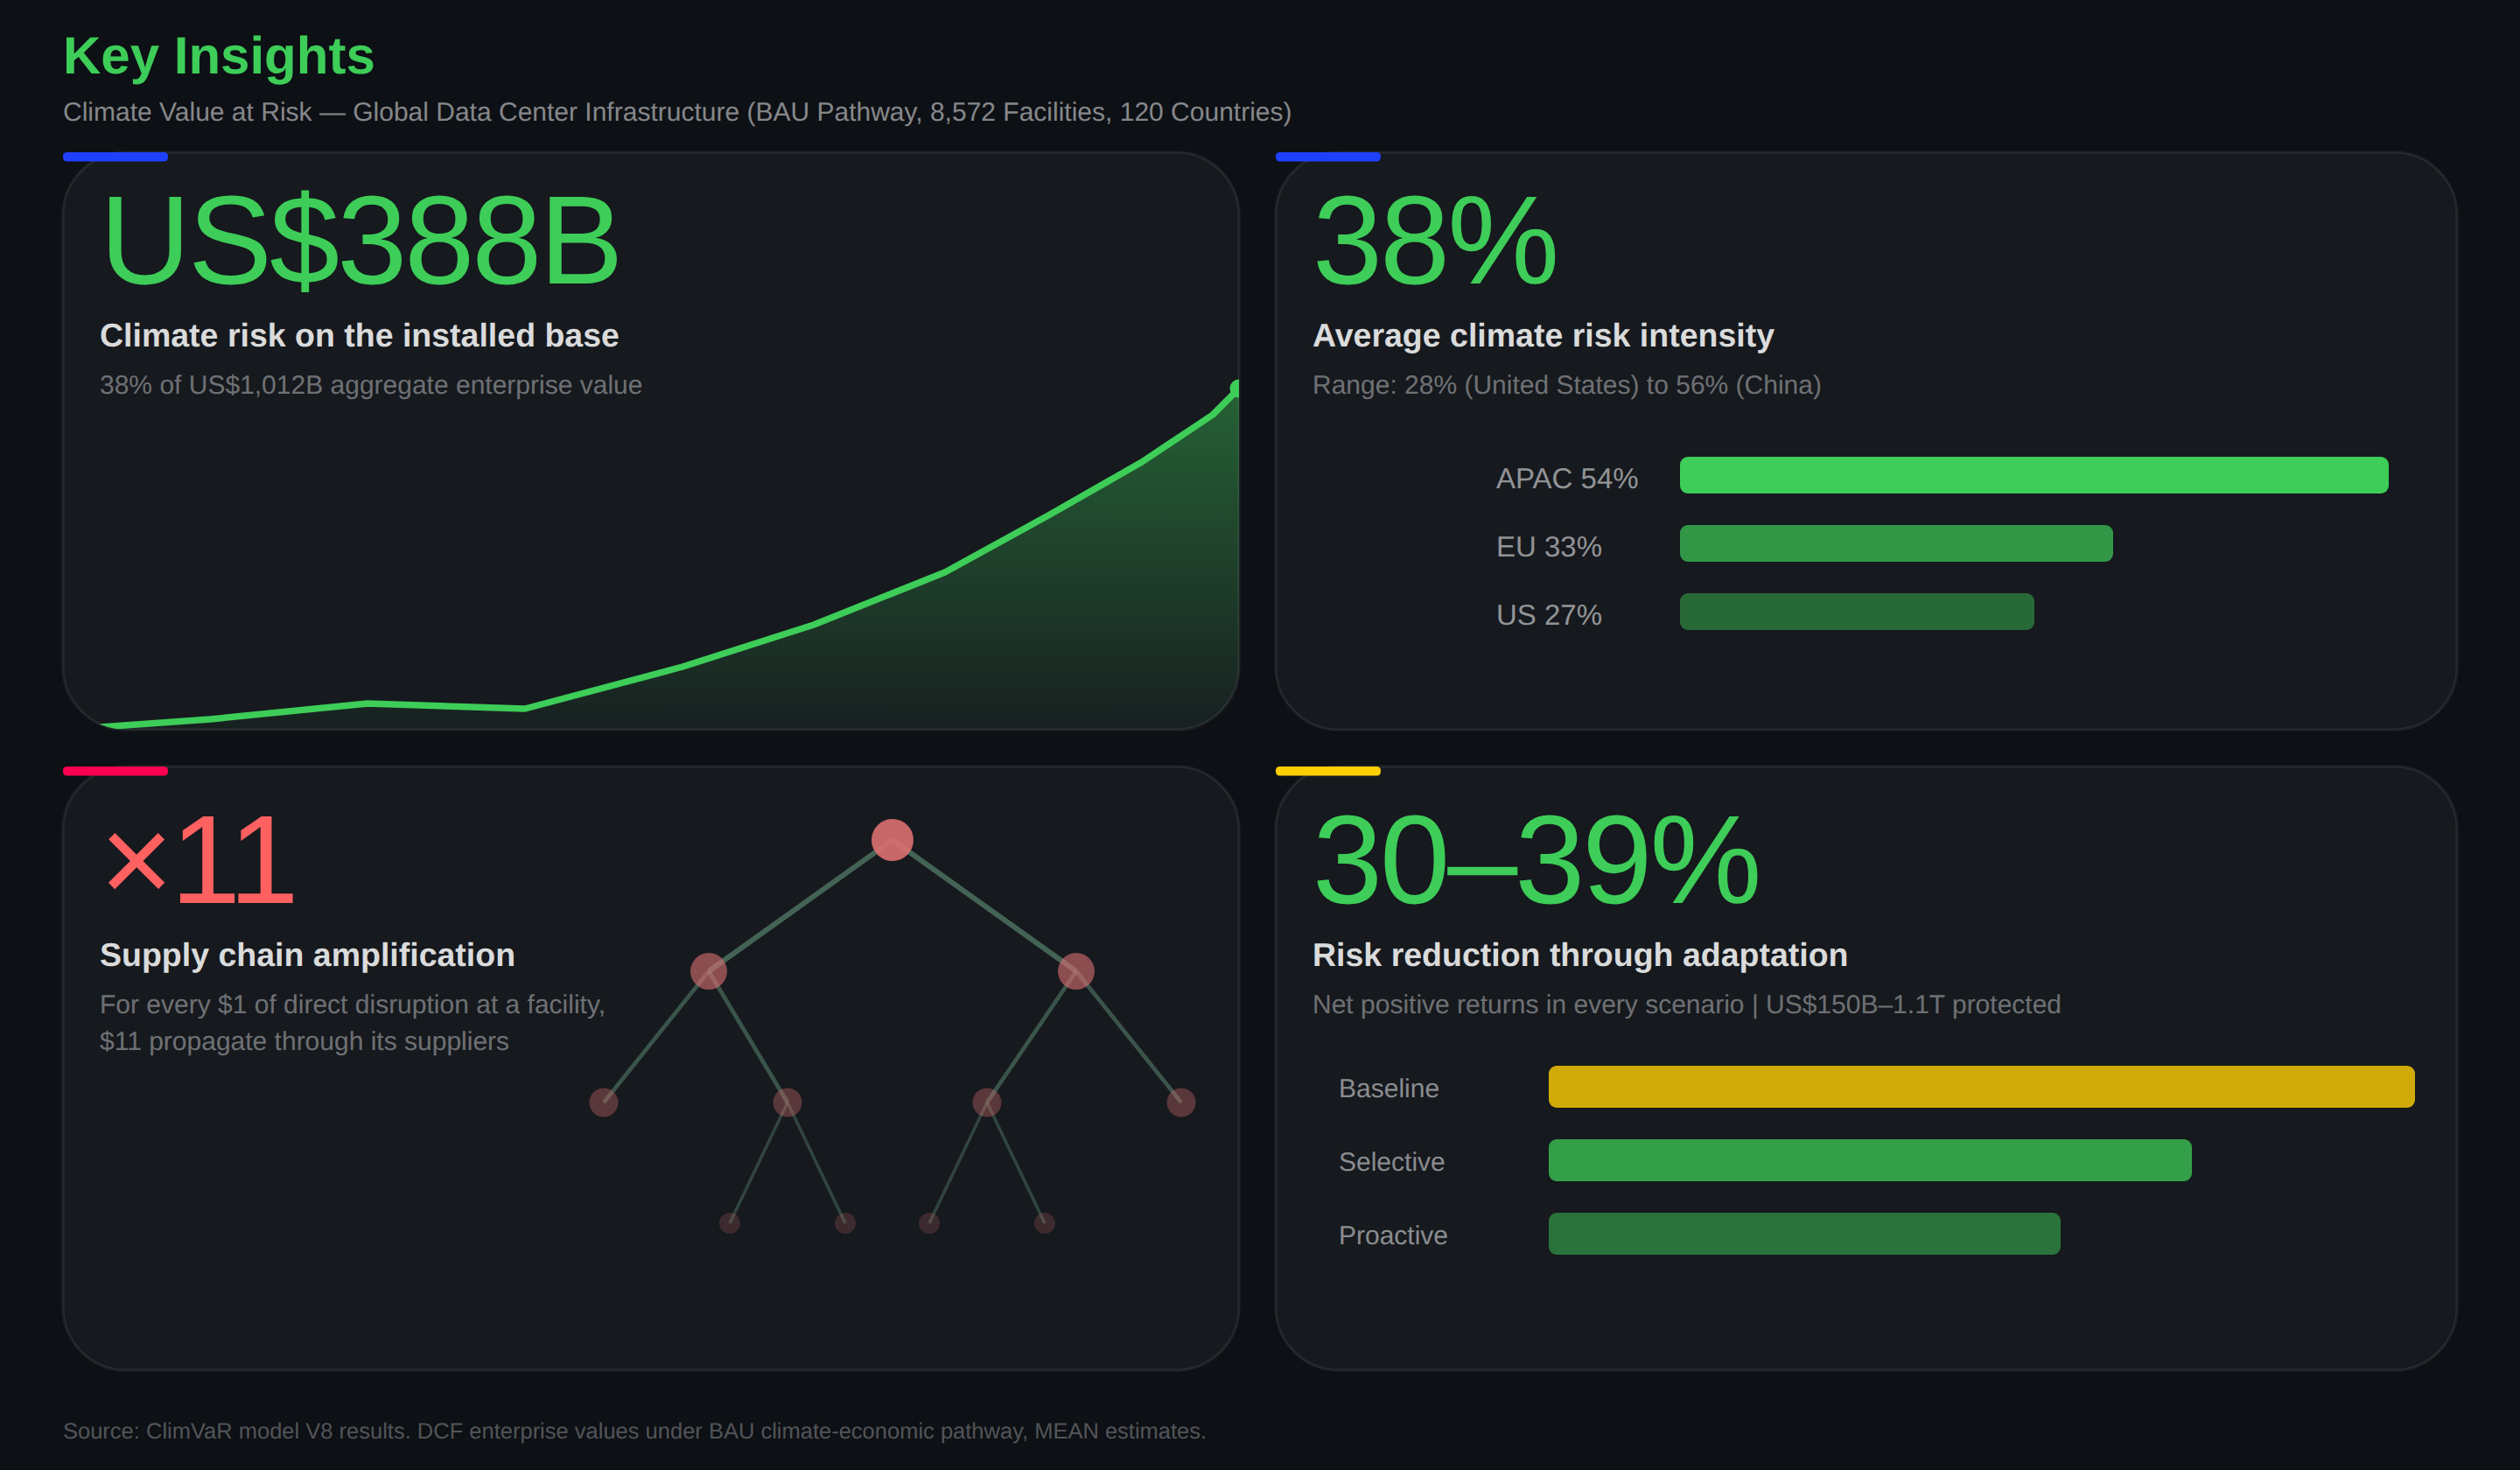
\includegraphics[width=\textwidth]{images/statstrip.png}
\end{center}

\vspace{2mm}

% --- Implications ---
{\displayfont\fontsize{13}{16}\selectfont\color{SEGreen}Implications\par}
\vspace{1mm}

\begin{multicols}{2}
\setlength{\parskip}{1pt}

\noindent{\fontsize{9}{11}\selectfont\textbf{\color{SEGreen}Capital markets \& financial modelling.}}\\[0pt]
Physical climate risk lacks anchor metrics equivalent to carbon intensity. Facility-level ClimVaR supplies the missing metric in a transparent format compatible with DCF models. Investors can price physical exposure into allocation, differentiate assets that look identical on paper, and identify mispriced opportunities before markets reprice them.

\vspace{1mm}

\noindent{\fontsize{9}{11}\selectfont\textbf{\color{SEGreen}Operators, system planners \& insurers.}}\\[0pt]
The same adaptation dollar generates 2--3$\times$ different returns depending on location and channel composition. Channel-level attribution identifies which lever matters most at each site. The $\times$11 supply chain multiplier reveals where systemic resilience pays off beyond the facility perimeter.

\vspace{1mm}

\noindent{\fontsize{9}{11}\selectfont\textbf{\color{SEGreen}AI developers \& hyperscalers.}}\\[0pt]
Sustainability strategies centered on renewable procurement address less than 10\% of AI-era climate exposure. Physical resilience, designed in at the front end, is both the binding constraint and the lever competitors are not yet pulling.

\vspace{1mm}

\noindent{\fontsize{9}{11}\selectfont\textbf{\color{SEGreen}Policymakers \& regulators.}}\\[0pt]
Data centers have shifted to strategic infrastructure, but climate exposure remains weakly integrated into permitting. A facility-level metric makes targeted policy possible: siting rules and stress tests calibrated to actual financial exposure.

\vspace{1mm}

\noindent{\fontsize{9}{11}\selectfont\textbf{\color{SEGreen}Chief sustainability officers.}}\\[0pt]
Climate reporting that stops at carbon captures only a quarter of exposure. The full five-channel picture turns a reporting obligation into a strategic instrument for resilience investment.

\end{multicols}
